\documentclass{article}%standalone can be used
\usepackage{tikz}
\usetikzlibrary{shapes.geometric, arrows, positioning}

\newcommand*{\boxWidth}{20mm}
\tikzset{
    point/.style     = {coordinate},
    arrow/.style     = {thick, ->, >=stealth'},
    to/.style        = {->,>=stealth', shorten >=1pt, semithick},
    decision/.style  = {draw, diamond, minimum width=\boxWidth, minimum height=10mm, text centered, aspect=2},
    process/.style   = {draw, rectangle, minimum width=\boxWidth, minimum height=10mm, text centered, text width=\boxWidth},
    startstop/.style = {draw, rectangle, rounded corners, minimum width=\boxWidth, minimum height=1cm,text centered, text width=\boxWidth}
}

\begin{document}
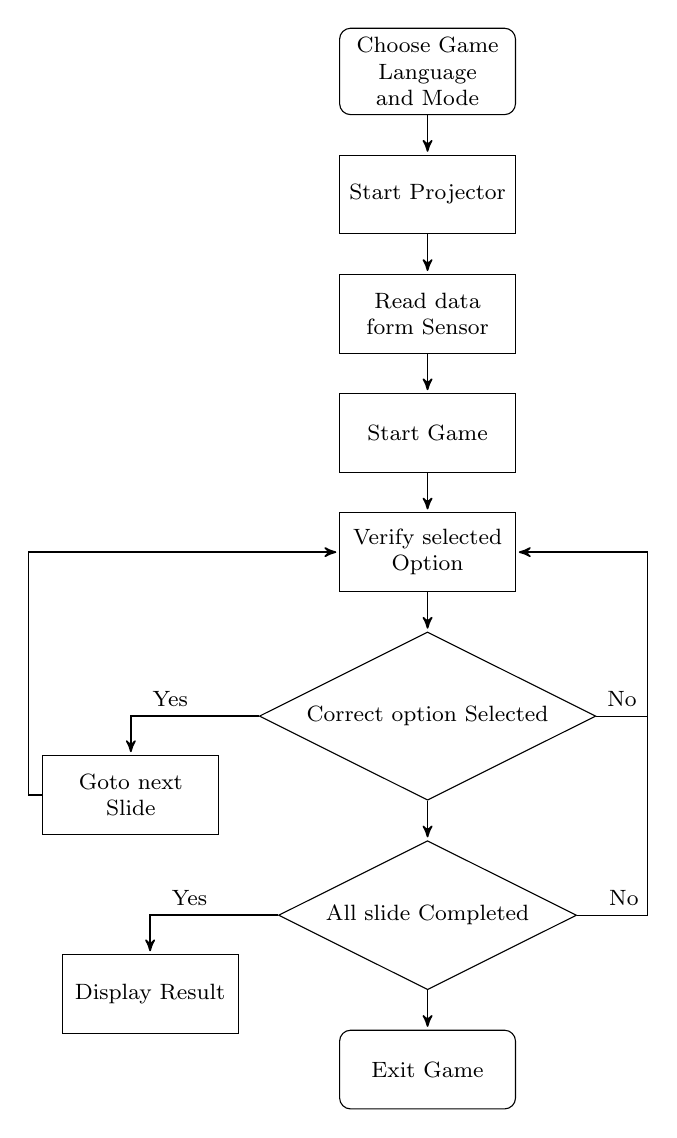
\begin{tikzpicture}[node distance=5mm, every node/.style={font=\footnotesize}]
	\node (start) [startstop] {Choose Game Language and Mode};
	\node (step1) [process, below=of start] {Start Projector};
	\node (step2) [process, below=of step1] {Read data form Sensor};
	\node (step3) [process, below=of step2] {Start Game};
	\node (step4) [process, below=of step3] {Verify selected Option};
	\node (step5) [decision, below=of step4] {Correct option Selected};
	\node (step5a)[point, right=of step5, xshift=1.5mm] {};
	\node (step5b)[process, left=of step5, yshift=-10mm] {Goto next Slide};
	\node (step6) [decision, below=of step5] {All slide Completed};
	\node (step7) [process, left=of step6, yshift=-10mm] {Display Result};
	\node (stop)  [startstop, below=of step6] {Exit Game};

	\draw [to] (start) -- (step1);
	\draw [to] (step1) -- (step2);
	\draw [to] (step2) -- (step3);
	\draw [to] (step3) -- (step4);
	\draw [to] (step4) -- (step5);
	\draw [-] (step5) -- node[above]{No}(step5a)coordinate(mid1);
	\draw [to] (mid1) |- (step4);
	\draw [to] (step5) -| node[above, xshift=5mm]{Yes}(step5b);
	\draw [to] (step5b) -- +(-13mm,0) |- (step4);
	\draw [to] (step5) -- (step6);
	\draw [to] (step6) -| node[above, xshift=5mm]{Yes}(step7);
	\draw [-] (step6) -| node[above, xshift=-3mm]{No}(mid1);
	\draw [to] (step6) -- (stop);
\end{tikzpicture}
\end{document}

